\section{Experiments}
\label{sec:exp}
We evaluate the efficiency and usefulness of \framework\ in an extensive set of experiments. We consider two types of experiments: first, a performance study measures the influence of relevance and size constraint thresholds on execution time. Second, we measure the usefulness of our framework in a user study.

\vspace{5pt}
\noindent {\bf Experiment Settings.} Unless otherwise stated, we use the same settings discussed in Section \ref{sec:scenarios}. All experiments are implemented in Python (functionality) and JavaScript D3 (visualization) on a 2.8GHz Intel Core i5 machine with an 16GB main memory, running OS X 10.9.2.

%\begin{figure}
%  \centering
%  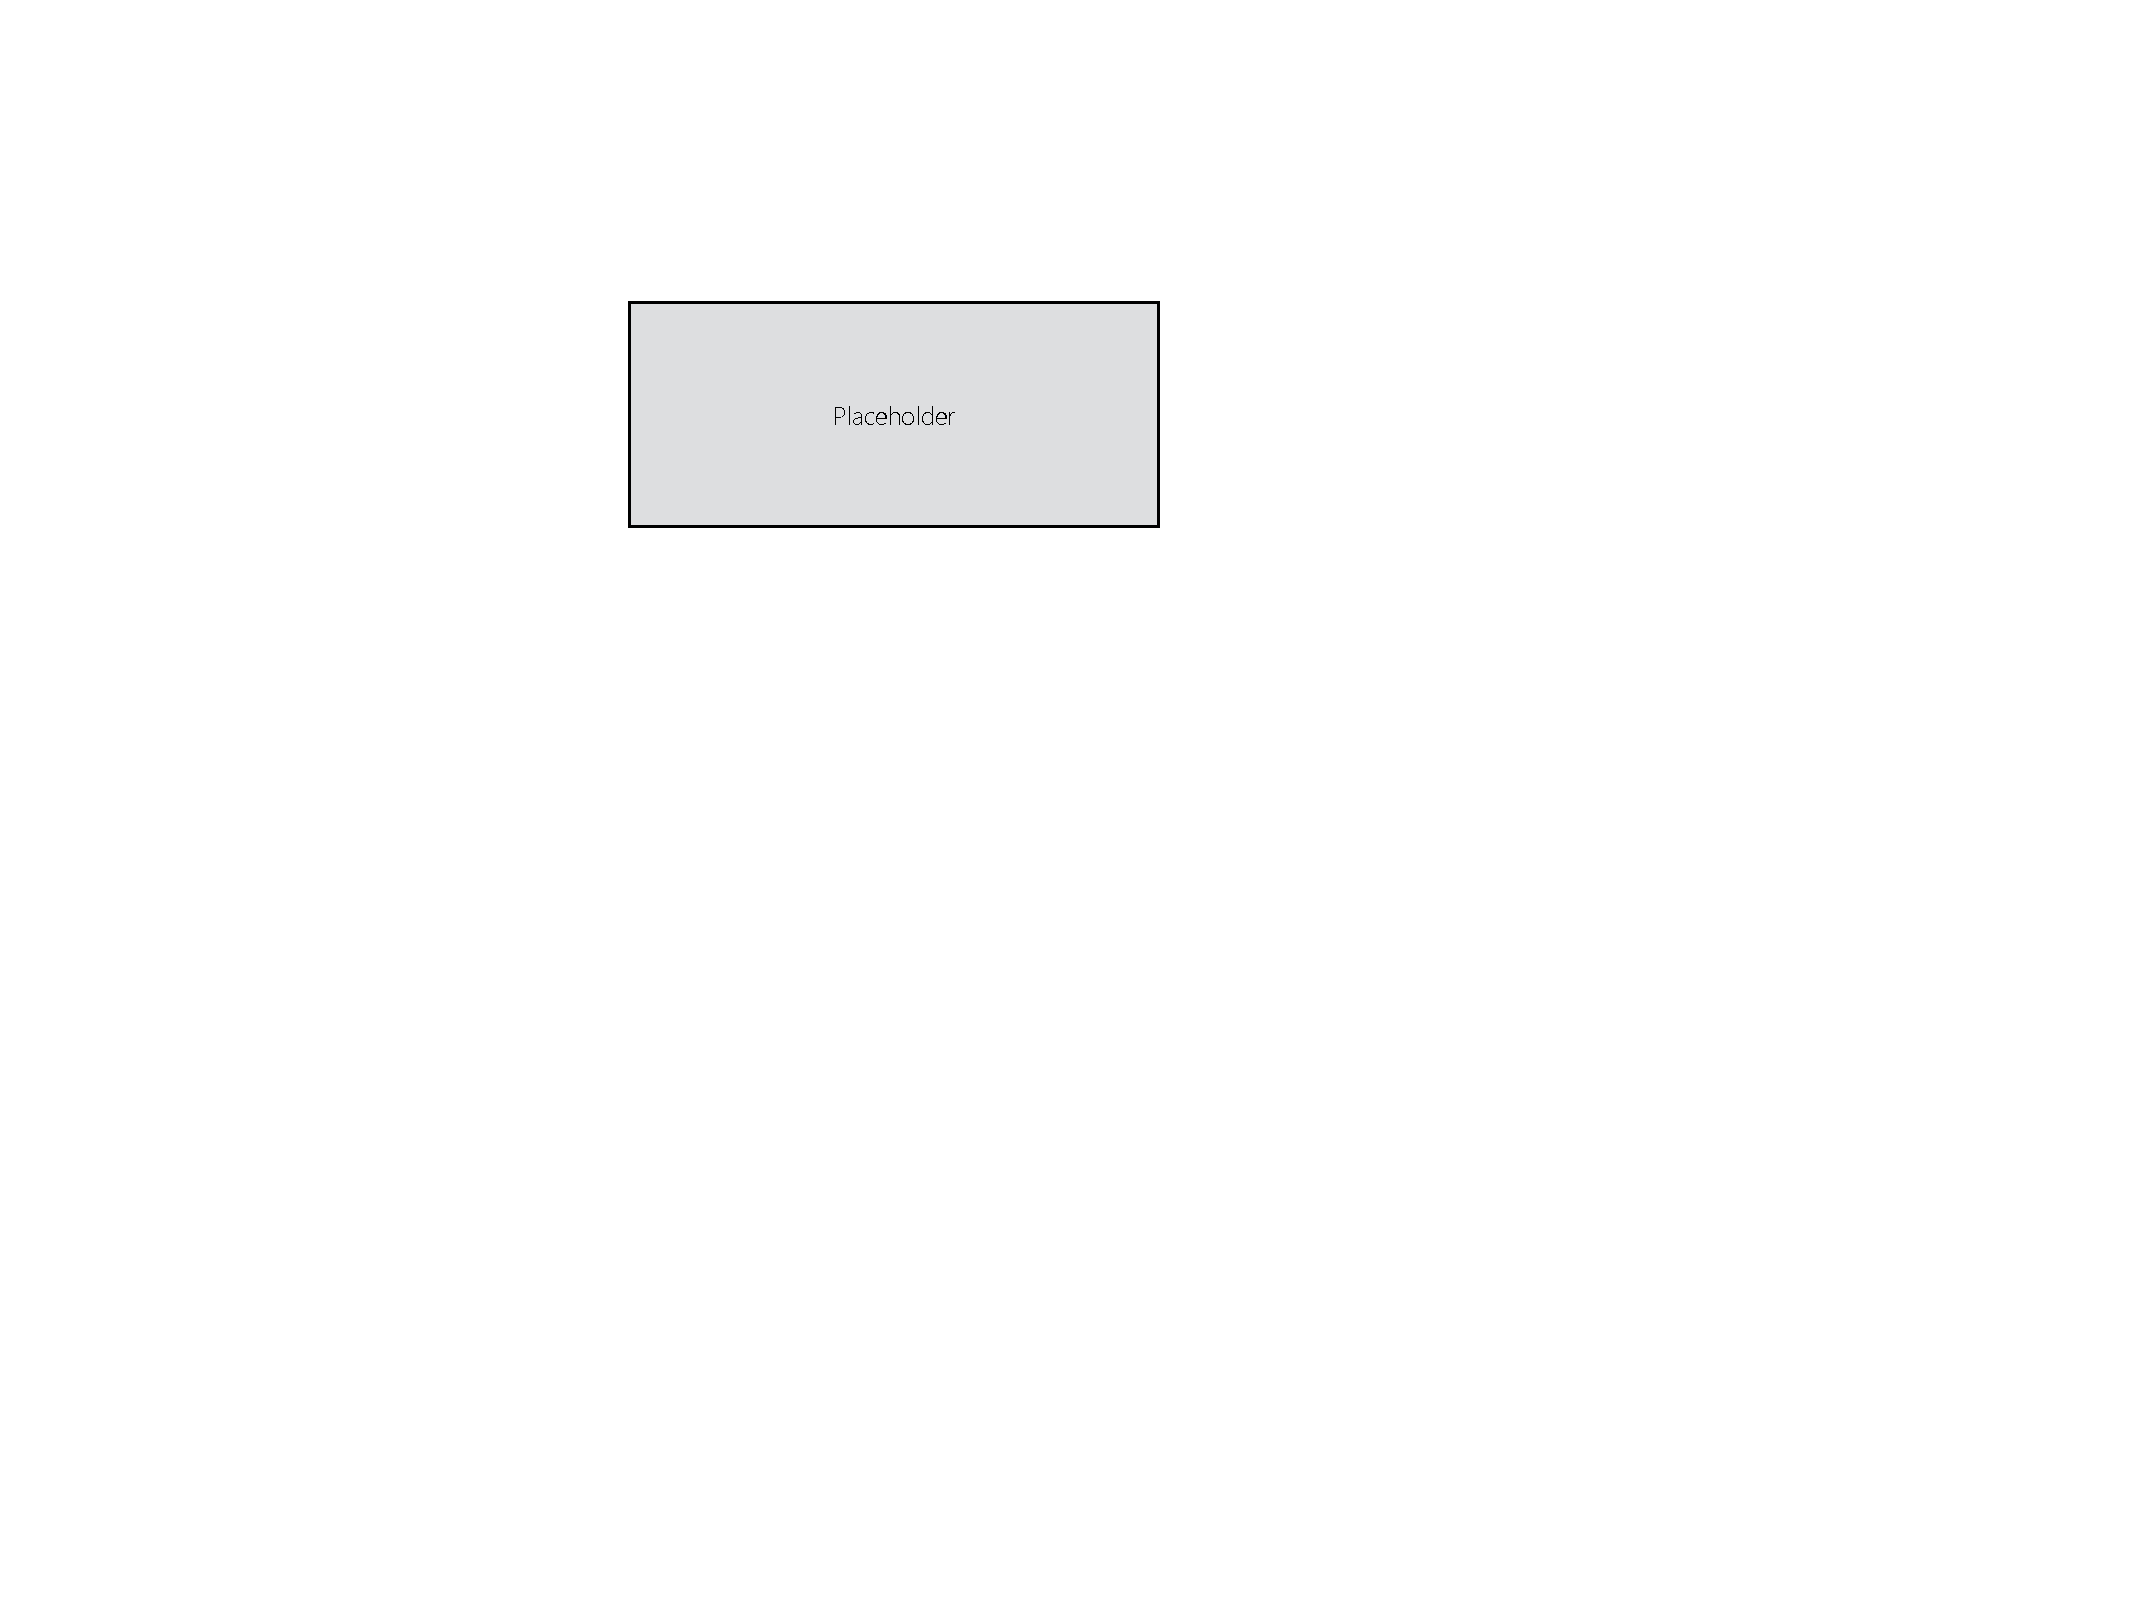
\includegraphics[width=\columnwidth]{figs/placeholder}
%\caption{Performance Evaluation}
%\label{fig:performance}
%\end{figure}

\begin{figure}
  \centering
<<<<<<< HEAD
% Preamble: 
\pgfplotsset{width=\columnwidth,compat=1.13}
\tiny
\begin{minipage}[b]{0.45\linewidth}
\begin{tikzpicture}
\begin{axis}[
	xlabel={Size Constraint (k)},
	ylabel={Similarity}
]

\addplot table [x=k, y=sim, col sep=comma] {figs/charts/c01/02.csv};
\addplot table [x=k, y=sim, col sep=comma] {figs/charts/c01/05.csv};
\addplot table [x=k, y=sim, col sep=comma] {figs/charts/c01/07.csv};
\addplot table [x=k, y=sim, col sep=comma] {figs/charts/c01/09.csv};

\tiny
%\legend{$\sigma=0.2$, $\sigma=0.5$, $\sigma=0.9$}
\end{axis}
\end{tikzpicture}
\end{minipage}
\hspace{0.2cm}
\begin{minipage}[b]{0.45\linewidth}
\begin{tikzpicture}
\begin{axis}[
	xlabel={Size Constraint (k)},
	ylabel={Diversity}
]

\addplot table [x=k, y=div, col sep=comma] {figs/charts/c01/02.csv};
\addplot table [x=k, y=div, col sep=comma] {figs/charts/c01/05.csv};
\addplot table [x=k, y=div, col sep=comma] {figs/charts/c01/07.csv};
\addplot table [x=k, y=div, col sep=comma] {figs/charts/c01/09.csv};
\tiny
%\legend{$\sigma=0.2$, $\sigma=0.5$, $\sigma=0.9$}
\end{axis}
\end{tikzpicture}
\end{minipage}

%%% SECOND LINE %%% 
\bigskip

\begin{minipage}[b]{0.45\linewidth}
\begin{tikzpicture}
\begin{axis}[
	%legend pos=outer north east,
	xlabel={Size Constraint (k)},
	ylabel={Time(sec)}
]

\addplot table [x=k, y=0.2, col sep=comma] {figs/charts/fig3.csv};
\addplot table [x=k, y=0.5, col sep=comma] {figs/charts/fig3.csv};
\addplot table [x=k, y=0.7, col sep=comma] {figs/charts/fig3.csv};
\addplot table [x=k, y=0.9, col sep=comma] {figs/charts/fig3.csv};
\tiny
%\legend{$\sigma=0.2$,$\sigma=0.5$,$\sigma=0.7$,$\sigma=0.9$}
\end{axis}
\end{tikzpicture}
\end{minipage}
\hspace{0.2cm}
\begin{minipage}[b]{0.45\linewidth}
\begin{tikzpicture}
\begin{axis}[
	%legend pos=outer north east,
	xlabel={Sigma ($\sigma$)},
	ylabel={Time(sec)}
]

\addplot table [x=sigma, y=2, col sep=comma] {figs/charts/fig4.csv};
\addplot table [x=sigma, y=100, col sep=comma] {figs/charts/fig4.csv};
\addplot table [x=sigma, y=200, col sep=comma] {figs/charts/fig4.csv};
\addplot table [x=sigma, y=300, col sep=comma] {figs/charts/fig4.csv};

\tiny
%\legend{$k=2$,$k=100$,$k=300$,$k=300$}
\end{axis}
\end{tikzpicture}
\end{minipage} 
  
=======
  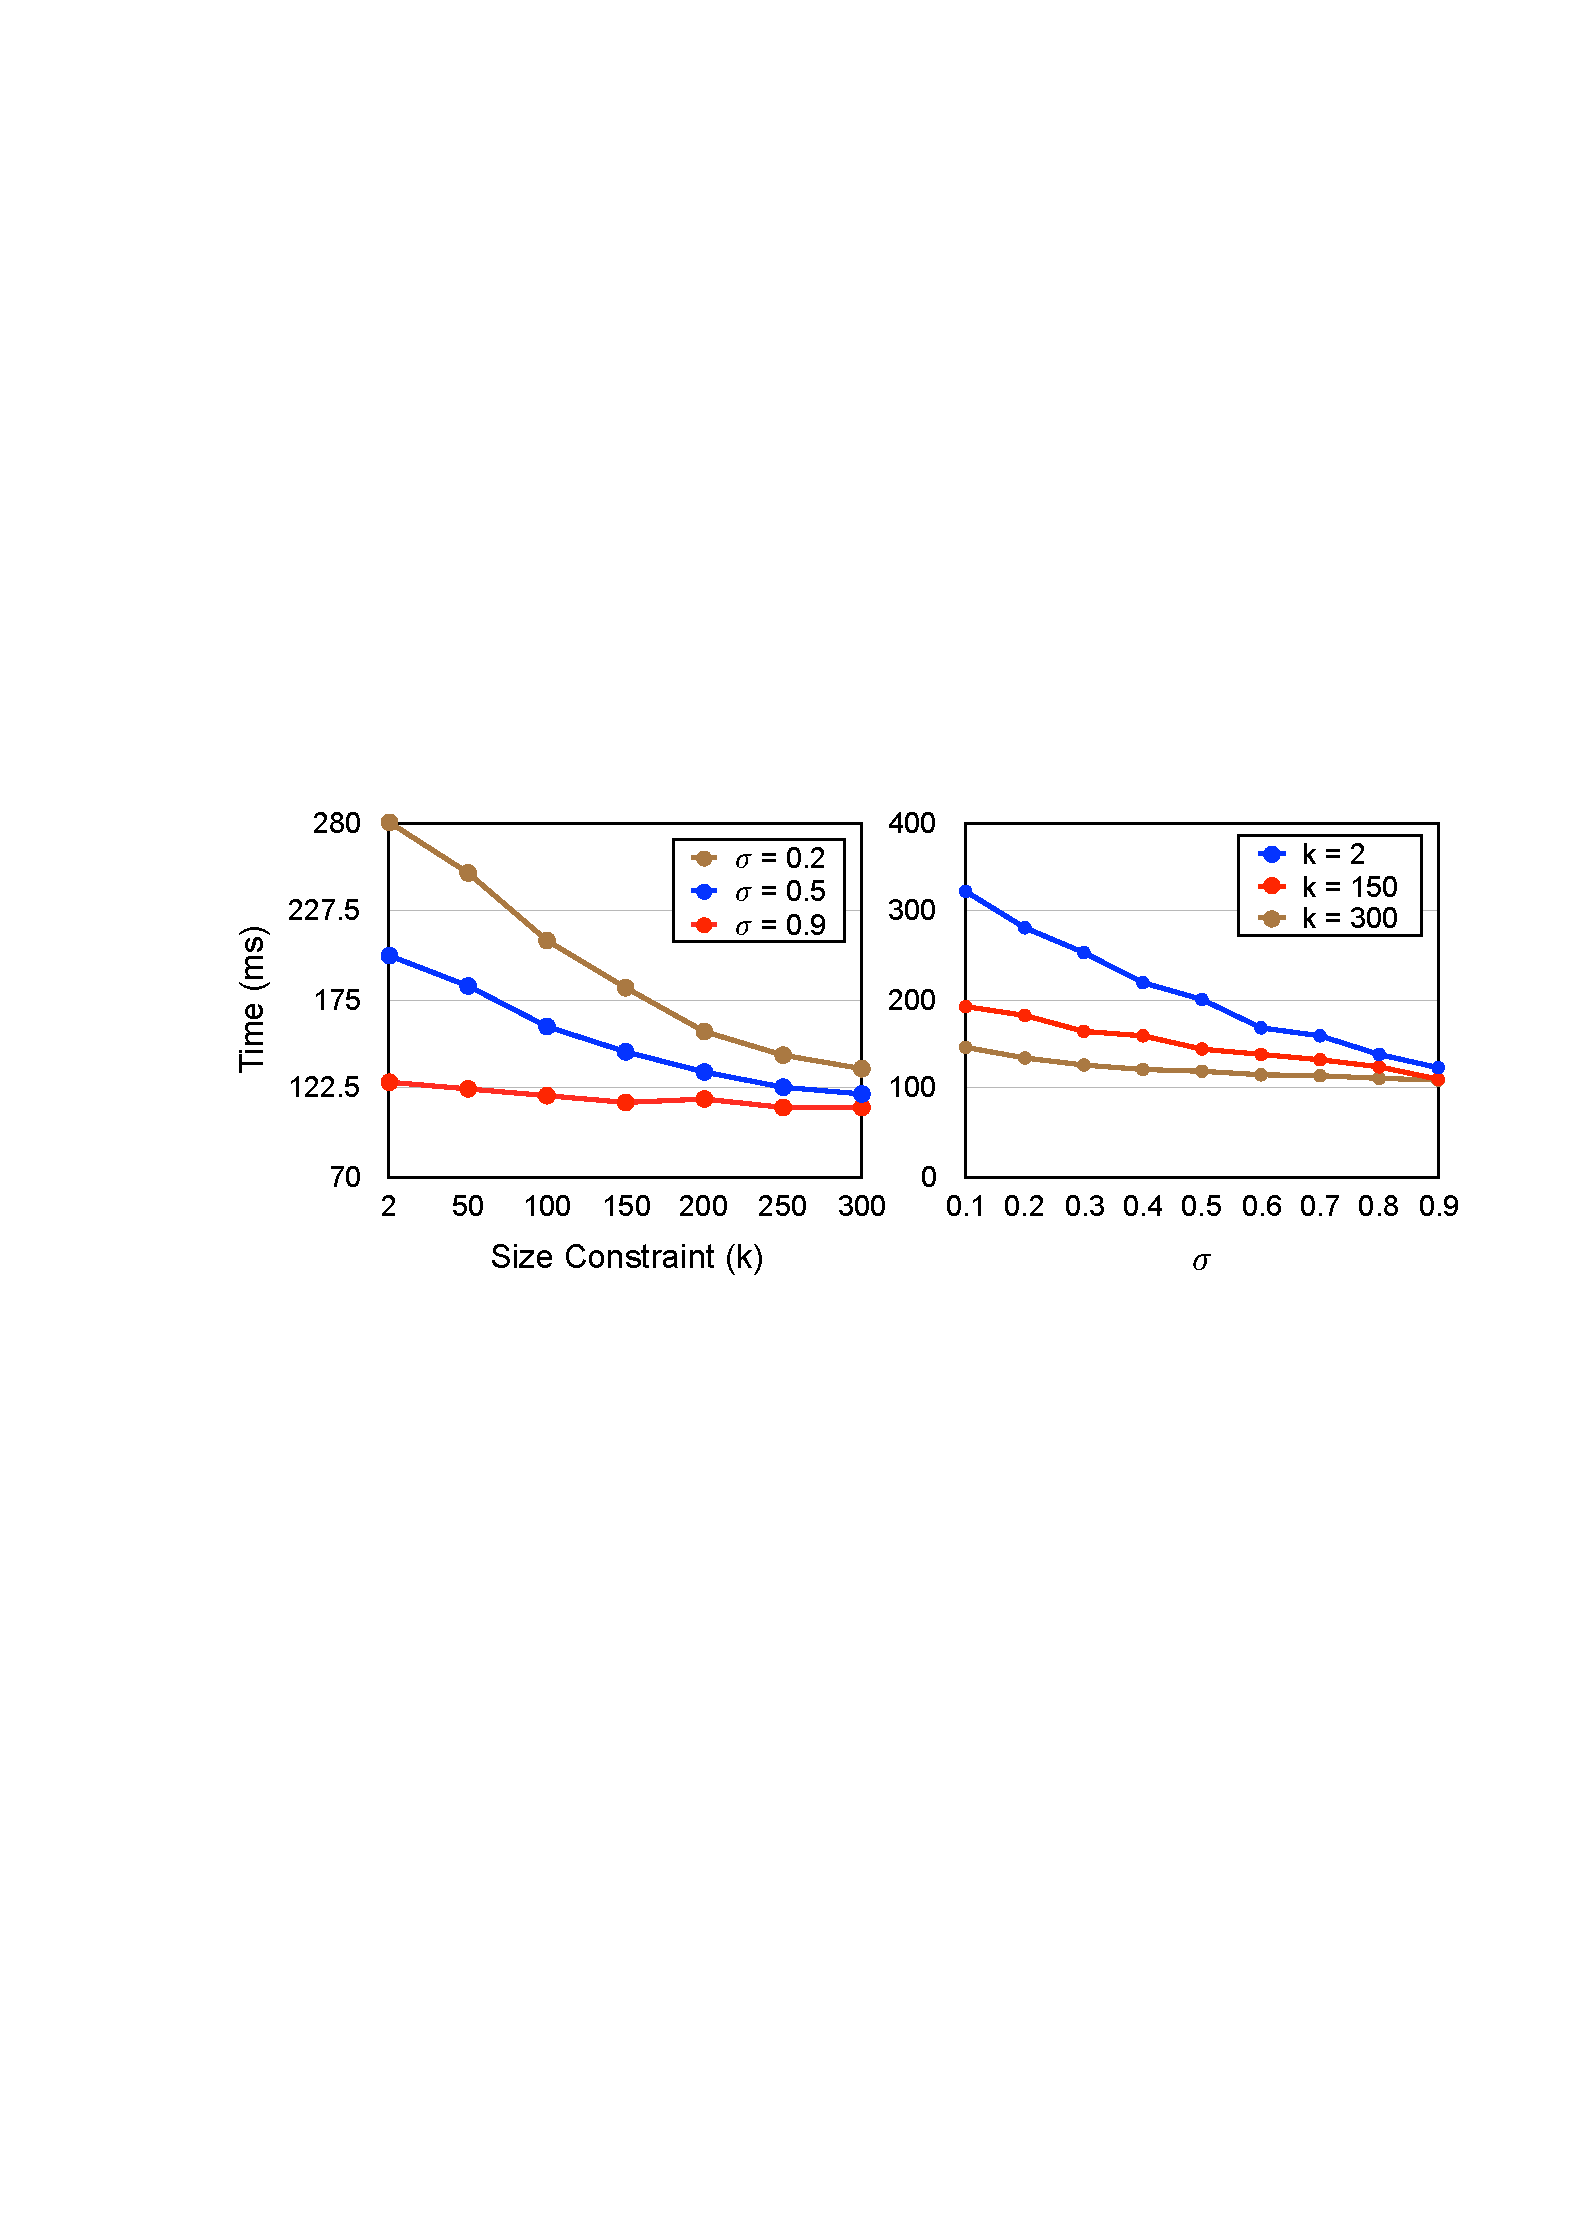
\includegraphics[width=\columnwidth]{figs/performance}
>>>>>>> master
\caption{Performance Evaluation}
\vspace{-10pt}
\label{fig:performance}
\end{figure}


<<<<<<< HEAD

=======
>>>>>>> master
\vspace{5pt}
\noindent {\bf Performance Study.} \framework\ is designed for exploratory context where interactivity is a need. The ``best-effort'' greedy approach of {\sc Highlighter} (Algorithm \ref{algo:geoh}) guarantees to return the best possible results within a time limit. We consider a large time limit ($tlimit = 2s$) in order to evaluate the effect of relevance and size constraint thresholds on execution time.
% Figure \ref{fig:performance} illustrates the results by measuring the execution time.

Figure \ref{fig:performance} left illustrates the effect of size constraint by varying $k$ from $2$ to $300$. Interestingly, we observe that increasing $k$ leads decreasing execution time. This is because in larger sets, there exist fewer opportunities for increasing diversity, hence {\sc Highlighter} breaks early. Figure \ref{fig:performance} right confirms that lower values of $\sigma$ decreases execution time as they provide more flexibility for diversity improvement.

\vspace{5pt}
\noindent {\bf User Study.}
The principled question that we ask ourselves is whether \framework\ is useful for analysts in practice. To answer this question, we designed a user study with $24$ participants (students in Computer Science). Half of the participants know the New York region well (experts) and the other half have a limited knowledge (novice). In our user study, we define a task for each participant and ask him/her to fulfill the task using both \framework\ and {\sc Tableau} (as the most advanced spatiotemporal visualization tool). Then we measure the cardinality of steps to reach the goal.

We define two tasks, {\em T1: finding a point in a requested location}, and {\em T2: finding a point with a requested profile}. As an example for {\em T1}, we ask participants to find points in the Central Park area. An example of {\em T2} is to find a drop-off point with \$2 tip whose trip distance is 3 kilometers. Participants may begin their navigation from three different starting points: {\em I1: close to the goal}, {\em I2: far from the goal}, and {\em I3: random}. We evaluate the effect of expertise, goal and starting point on the analysis length. Figure \ref{fig:userstudy} illustrates the results for novice (left) and expert (right) participant.

We observe that in general, it takes in average 10.7 steps to reach a defined goal in \framework, i.e., 33 steps less than {\sc Tableau}. This shows that the guidance component helps analysts discover their data and quickly reach to the goal. Level of expertise improves the analysis length in average by 4 steps. Interestingly, starting points do not have a huge influence. It is potentially due to the diversity component which provides distinct options. We also observe that {\em T2} is an easier task than {\em T1}. This is potentially due to similarity component where the analyst can request options similar to what she has already seen and greedily moves to match profiles.

\begin{figure}[t]
 \centering
 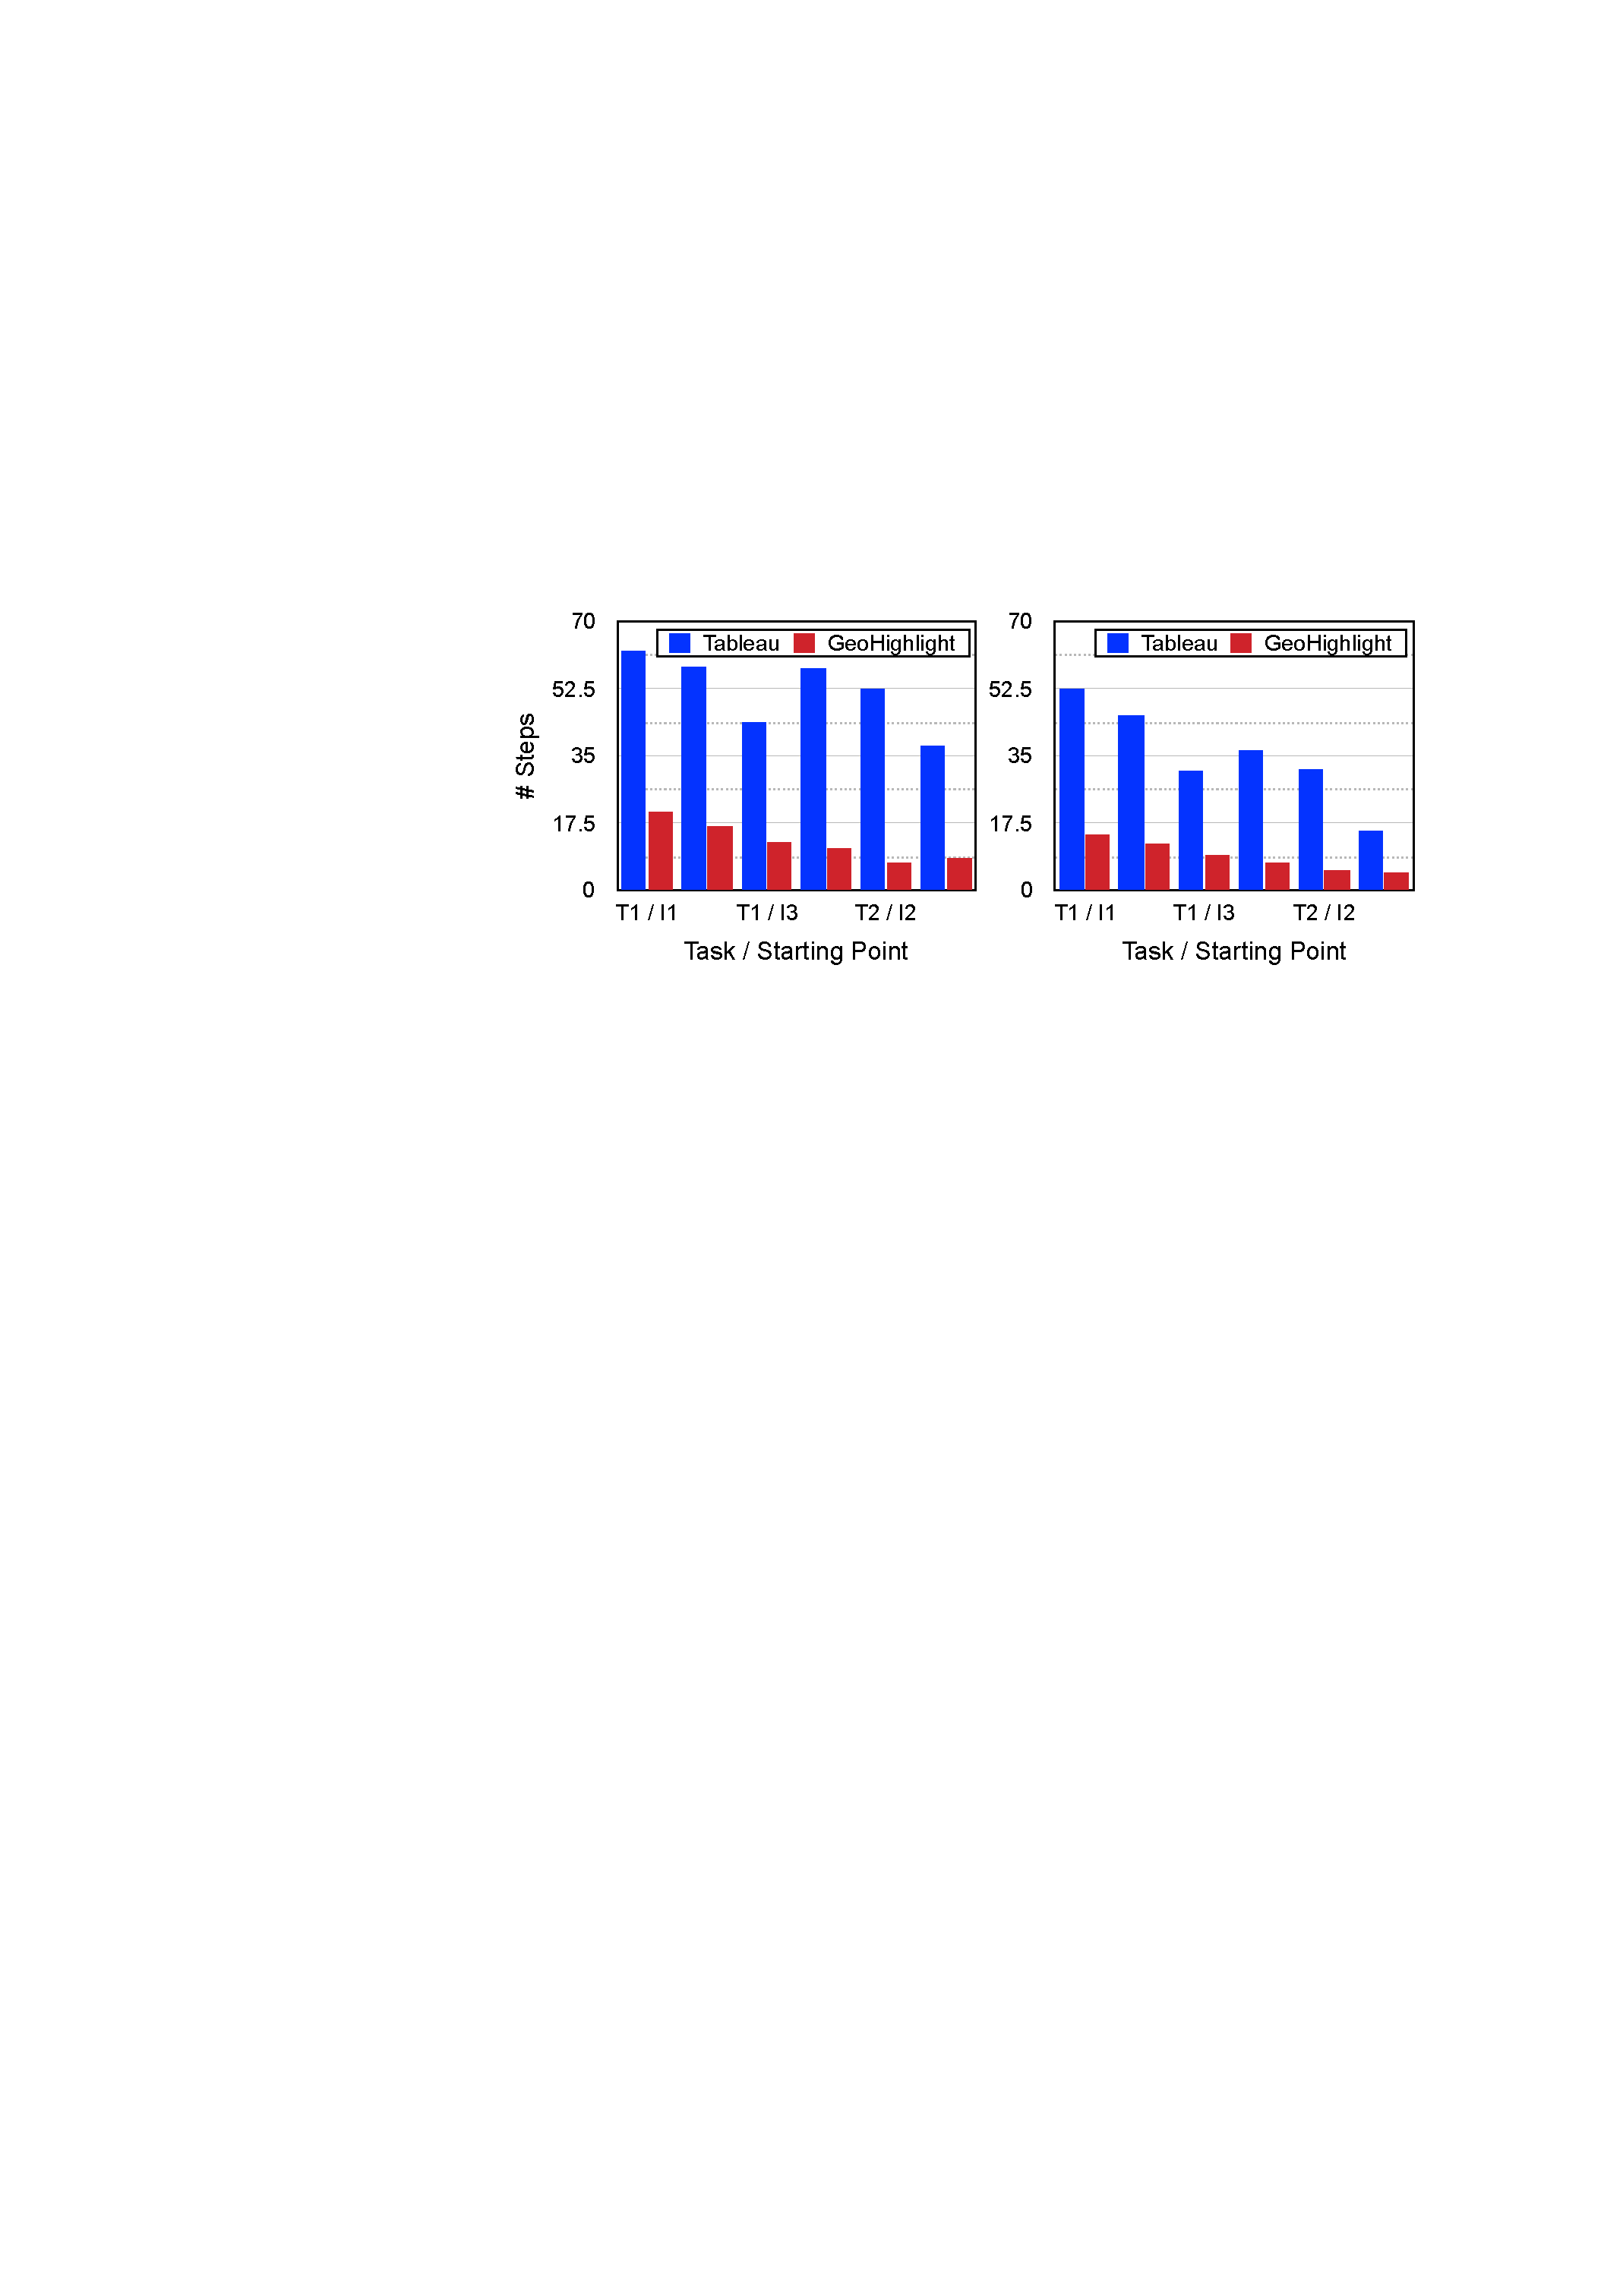
\includegraphics[width=\columnwidth]{figs/userstudy}
\caption{User Study}
\vspace{-5pt}
\label{fig:userstudy}
\end{figure}

% We also asked our participants about their insights on \framework. We ask them to rate the following metric on a 5-star scale: {\em usefulness} and {\em ease-of-use}. In summary, we found that \colorred{[explain received results]}.